\chapter{Aprendizaje Automático}
%

El Aprendizaje Automático, conocido en inglés como \textit{Machine Learning}, representa una de las áreas más dinámicas y prometedoras dentro del campo de la inteligencia artificial contemporánea. se fundamenta en el desarrollo de algoritmos y modelos computacionales capaces de identificar patrones complejos en conjuntos de datos, con el propósito de generar predicciones o tomar decisiones informadas sin necesidad de instrucciones programáticas explícitas para cada escenario específico.[]
%

La esencia del aprendizaje automático radica en su capacidad para mejorar el desempeño de manera iterativa mediante la experiencia acumulada. Mitchell proporciona una definición operacional particularmente esclarecedora: un sistema computacional manifiesta capacidad de aprendizaje cuando su rendimiento en una tarea determinada T, cuantificado mediante una métrica de desempeño P, experimenta una mejora mensurable como consecuencia de la exposición a una experiencia E.[] Esta conceptualización establece tres componentes fundamentales que articulan cualquier sistema de aprendizaje automático: la tarea objetivo, la experiencia de aprendizaje y el criterio de evaluación.
%

Para ilustrar estos conceptos de manera concreta, se puede examinar el caso de los sistemas de filtrado de correo electrónico no deseado. Un filtro de spam ejemplifica de forma paradigmática los principios del aprendizaje automático. El sistema desarrolla progresivamente la capacidad de discriminar entre mensajes legítimos y correo no solicitado mediante el análisis de ejemplos previamente etiquetados por usuarios. Estos conjuntos de datos, denominados conjuntos de entrenamiento, contienen tanto instancias positivas (correos identificados como spam) como negativas (mensajes legítimos), permitiendo al algoritmo extraer características distintivas de cada categoría.
%

En este contexto específico, la tarea T consiste en la clasificación binaria de nuevos mensajes electrónicos, la experiencia E está constituida por el proceso de entrenamiento con los datos etiquetados, y la métrica de desempeño P puede definirse como la tasa de precisión o \textit{Accuracy}, que cuantifica la proporción de mensajes correctamente clasificados en relación con el total de predicciones realizadas.
%

\section{Clasificación de sistemas o tipos de aprendizaje automático}
%

La diversidad de aplicaciones y contextos en los que se implementan sistemas de aprendizaje automático ha propiciado el desarrollo de múltiples paradigmas metodológicos. La clasificación más fundamental de estos enfoques se establece en función del tipo y grado de supervisión disponible durante la fase de entrenamiento. A continuación, se muestran las tres categorías principales:
%

\begin{itemize}
    \item \textbf{Aprendizaje supervisado:} Este paradigma constituye el enfoque más ampliamente implementado en aplicaciones prácticas. Se caracteriza por la disponibilidad de un conjunto de entrenamiento que incluye pares de entrada-salida, donde cada instancia de entrada está asociada con su correspondiente etiqueta o \textit{label}, que representa la solución correcta. El objetivo del algoritmo consiste en inferir una función de mapeo que establezca la correspondencia óptima entre el espacio de características de entrada y el conjunto de salidas deseadas, de manera que pueda generalizar efectivamente a instancias no observadas previamente.
    
    El aprendizaje supervisado se subdivide en dos categorías fundamentales según la naturaleza de la variable objetivo:

    \begin{itemize}
        \item \textit{Clasificación:} Se trata de brindar ejemplos de entrenamiento donde cada instancia está asociada con una o múltiples clases predefinidas, a modo de que se pueda realizar el entrenamiento y clasificar nuevas entradas dentro de alguna de las clases existentes. Aplicaciones típicas incluyen el reconocimiento de imágenes, detección de fraudes y análisis de sentimientos.
        
        \item \textit{Predicción:} A diferencia de la clasificación, éste consiste en la predicción de una variable objetivo de naturaleza continua o numérica. El sistema recibe datos de entrenamiento compuestos por vectores de características junto con sus valores objetivos correspondientes, permitiendo al modelo aprender la relación funcional entre sí. Esta capacidad predictiva se aplica posteriormente para estimar valores numéricos de nuevas instancias basándose exclusivamente en sus características de entrada. Aplicaciones típicas comprenden la predicción de precios, estimación de demanda y proyecciones temporales.
    \end{itemize}
    
    \item \textbf{Aprendizaje no supervisado:} Este paradigma aborda escenarios donde los datos de entrenamiento carecen de soluciones deseadas. La ausencia de supervisión directa plantea un desafío metodológico fundamentalmente diferente: el algoritmo debe descubrir estructuras intrínsecas, patrones latentes o relaciones subyacentes en los datos sin guía externa. Las técnicas de aprendizaje no supervisado resultan particularmente valiosas para tareas exploratorias, tales como la segmentación de clientes, detección de anomalías, reducción de dimensionalidad y descubrimiento de asociaciones en grandes volúmenes de datos. Este enfoque refleja una aproximación más cercana a cómo los sistemas biológicos pueden aprender mediante la observación y organización autónoma de información sensorial.
    
    \item \textbf{Aprendizaje por refuerzo:} Este paradigma se distingue por su naturaleza secuencial e interactiva. En lugar de aprender a partir de un conjunto estático de ejemplos, el aprendizaje por refuerzo se fundamenta en la interacción continua de un agente con un entorno dinámico. El proceso de aprendizaje se articula mediante señales de retroalimentación en forma de recompensas (positivas o negativas) que el agente recibe como consecuencia de sus acciones. El objetivo fundamental consiste en desarrollar una política de comportamiento que maximice la recompensa acumulada a largo plazo.
     Este bucle de retroalimentación continua entre acción, observación y recompensa permite al sistema refinar progresivamente su estrategia mediante exploración y explotación del espacio de estados. Las aplicaciones emblemáticas incluyen sistemas de control robótico, estrategias de juegos, optimización de recursos y vehículos autónomos.
\end{itemize}
%

Cada uno de estos paradigmas presenta ventajas distintivas y limitaciones inherentes, determinando su idoneidad para contextos específicos. La selección del enfoque apropiado constituye una decisión metodológica crucial que debe considerar tanto la naturaleza del problema como las características de los datos disponibles.
%

\section{Redes Neuronales Artificiales}
%

Las redes neuronales artificiales constituyen una clase de algoritmos computacionales bio-inspirados que emulan, de manera simplificada, la arquitectura y funcionamiento del sistema nervioso biológico. Al igual que en el cerebro, estas estructuras computacionales se componen de unidades elementales denominadas neuronas artificiales, las cuales establecen conexiones entre sí formando redes complejas. Cada neurona recibe señales de entrada, las procesa mediante funciones matemáticas específicas y transmite el resultado a otras neuronas de la red, operando de manera análoga a un interruptor que se activa bajo determinadas condiciones.
%

La potencia computacional de las redes neuronales artificiales no reside en la sofisticación de sus componentes individuales, sino en la emergencia de comportamientos complejos producto de las interacciones masivas entre múltiples unidades simples. Esta propiedad refleja un principio fundamental observado en sistemas biológicos: el cerebro humano, con aproximadamente cien mil millones de neuronas y cien billones de sinapsis, genera capacidades cognitivas extraordinarias a partir de la interconexión de elementos relativamente simples. De manera similar, las redes neuronales artificiales derivan su capacidad de aprendizaje y generalización de la organización colectiva de sus unidades, más que de la complejidad algorítmica de cada neurona individual.
%

\subsection{Perceptrón}
%

El perceptrón constituye la unidad computacional elemental de las redes neuronales artificiales, inspirado directamente en el funcionamiento de las neuronas biológicas. Estas células nerviosas operan mediante un mecanismo de umbralización: reciben señales eléctricas de múltiples fuentes y, cuando la suma de estos estímulos supera un umbral crítico, generan un potencial de acción que se propaga a neuronas subsecuentes.
%

\begin{figure}[H]
    \centering
    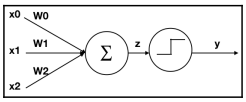
\includegraphics{capitulos/img/perceptron.png}
    \caption{Comportamiento del perceptrón}
    \label{fig:perceptron}
\end{figure}
%

El perceptrón emula este comportamiento mediante un modelo matemático relativamente simple, como se ilustra en la figura \ref{fig:perceptron}. Este componente puede recibir múltiples señales de entrada representadas por el vector \(X = \{x_{0},x_{1},x_{2},...,x_{n}\}\). Cada entrada es ponderada mediante multiplicación con un peso correspondiente del vector \(W = \{w_{0},w_{1},w_{2},...,w_{n}\}\). La suma ponderada resultante, denotada como \(z\), se procesa posteriormente mediante una función de activación que determina la salida final \(y\). Este proceso puede expresarse formalmente como:
%

\begin{equation}
z = \sum_{i=1}^{n} w_{i} x_{i} = w^{T}x
\end{equation}
%

Esta ecuación presenta dos representaciones equivalentes del modelo neuronal: la suma explícita de productos y su formulación vectorial compacta. El término \(w^{T}x\) denota el producto escalar entre el vector de pesos transpuesto y el vector de entradas. Para completar la descripción matemática, se incorpora un término de sesgo \textit{b} o \textit{bias}:
%

\begin{equation}
z = \sum_{i=1}^{n} w_{i} x_{i} + b = w^{T}x + b
\end{equation}
%

Esta expresión representa una combinación lineal de las entradas, que constituye la etapa previa a la aplicación de la función de activación. La función de activación determina la respuesta final del perceptrón ante los estímulos recibidos.
%

Existen diversas funciones de activación según la aplicación específica. La más elemental es la función escalón o función de paso, que produce una salida binaria definida por:
%

\begin{equation}
f(x)=\left\lbrace\begin{array}{c} 1~~~\text{si}~ (w^{T} x+b) > 0 \\ 0~~~\text{caso contrario} \end{array}\right.
\end{equation}
%

Esta función implementa una decisión de umbral simple, donde el perceptrón se activa únicamente cuando la combinación lineal de sus entradas excede cero.
%

\subsection{Funciones de activación}
%

Las funciones de activación son componentes esenciales que determinan la salida de cada neurona según su entrada. Su principal propósito es introducir no-linealidad en el modelo, aspecto crucial dado que sin ellas, la composición de múltiples capas lineales equivaldría a una única transformación lineal, limitando severamente la capacidad representacional de la red.
%

Entre las funciones más utilizadas se encuentran la sigmoide, la tangente hiperbólica (tanh) y la unidad lineal rectificada (ReLU, \textit{rectified linear unit}), cada una con características específicas según la aplicación, como se observa en la figura \ref{fig:funcionesActivacion}.
%

\begin{figure}[h!]
    \centering
    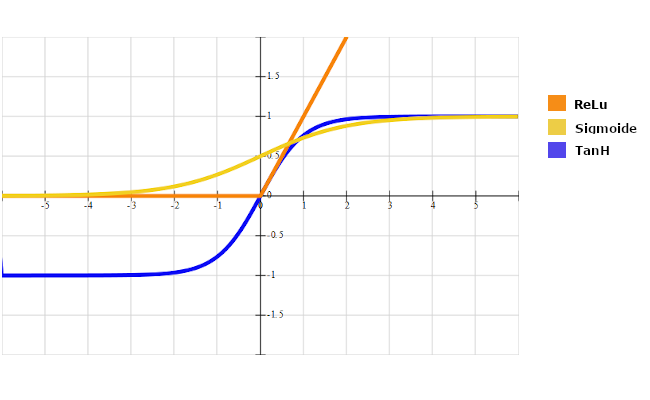
\includegraphics[width=1\textwidth]{capitulos/img/funcion_activacion.png}
    \caption{Funciones de Activación}
    \label{fig:funcionesActivacion}
\end{figure}
%

\newpage
\subsection{Arquitectura y aprendizaje}
%

La interconexión de múltiples neuronas artificiales configura una red neuronal. En las arquitecturas convencionales, las neuronas se organizan en capas, donde cada unidad está conectada a todas las neuronas de las capas adyacentes mediante conexiones ponderadas.
%

La figura \ref{fig:redNeuronal} ilustra una arquitectura típica estructurada en tres componentes. La capa de entrada recibe y alimenta los datos al sistema. Las capas intermedias u ocultas realizan transformaciones progresivas de la información; su número determina la profundidad de la red. La capa de salida genera las predicciones finales, con una dimensionalidad que depende del problema: una neurona para regresión o clasificación binaria, múltiples neuronas para clasificación multiclase.
%

\begin{figure}[H]
    \centering
    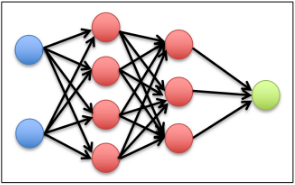
\includegraphics{capitulos/img/redNeuronal.png}
    \caption{Ejemplo de red neuronal}
    \label{fig:redNeuronal}
\end{figure}
%

Una vez establecidos los pesos de las conexiones de la red, es posible calcular valores de salida para cualquier entrada. Inicialmente, estos pesos se asignan de manera aleatoria, por lo que las salidas calculadas difieren de los valores esperados. El objetivo consiste en ajustar individualmente estos pesos para minimizar el error cuadrático medio entre las predicciones y los valores reales, proceso realizado mediante el método de retropropagación o \textit{backpropagation}.
%

El procedimiento opera de la siguiente manera: se calcula la salida para un registro del conjunto de datos y se determina el error respecto al valor esperado. Este error se propaga hacia atrás a través de todas las capas, desde la capa de salida hasta la capa de entrada, ajustando los pesos en función de su contribución al error total. Este proceso se repite iterativamente para cada registro del conjunto de datos.
%

La minimización del error se realiza mediante el método de descenso del gradiente, ambos algoritmos se explican detalladamente en \cite{[]}.
%

El ratio de aprendizaje o \textit{Learning Rate} determina la magnitud de los ajustes aplicados a los pesos en cada iteración. Un valor alto acelera la convergencia pero puede comprometer la precisión, mientras que un valor bajo favorece una convergencia más estable aunque más lenta. Los valores típicamente empleados oscilan entre 0.001 y 0.3.
%

El entrenamiento con una única pasada del conjunto de datos resulta insuficiente para alcanzar el mínimo error, especialmente con valores bajos de \textit{Learning Rate}. Por ello, se realizan múltiples iteraciones completas del conjunto de datos a través de la red, denominando a cada pasada completa como época o \textit{epoch}.
%

\section{Aplicación de Machine Learning en Redes Ópticas Elásticas Multinúcleo}
%

En esta sección se presenta un estudio bibliográfico del estado del arte de técnicas de \textit{Machine Learning} aplicadas a problemas en redes ópticas elásticas multinúcleo (MC-EON, \textit{Multi-Core Elastic Optical Networks}).
%

Panchali Datta Choudhury y Tanmay De presentan un análisis comprehensivo del uso de técnicas de \textit{Machine Learning} en redes ópticas elásticas \cite{[]}, fundamento que se extiende a las arquitecturas multinúcleo. Las MC-EON introducen complejidades adicionales respecto a las redes ópticas elásticas convencionales, particularmente en la gestión de múltiples núcleos dentro de una misma fibra y los fenómenos de interferencia entre núcleos (inter-core crosstalk), aspectos que requieren estrategias de optimización más sofisticadas donde el \textit{Machine Learning} demuestra particular utilidad.
%

Las principales áreas de aplicación de estas técnicas en el contexto de MC-EON incluyen:
%


\begin{itemize}
    \item Evaluación y predicción de calidad de servicio
    
    La investigación presentada en \cite{[]} propone un modelo de asignación de ancho de banda en EON considerando los requisitos de calidad de servicio o \textit{Quality of Service} (QoS). Se emplea aprendizaje por refuerzo o \textit{Reinforcement Learning}, donde la función de recompensa se fundamenta en el cumplimiento de los requisitos de QoS. En el contexto de MC-EON, esta aproximación adquiere mayor relevancia debido a la necesidad de garantizar QoS considerando simultáneamente la asignación de recursos en múltiples núcleos y la gestión de interferencias entre ellos.
    
    \item Supervivencia de red
    
    El trabajo presentado en \cite{[]} explora la optimización de redes considerando su capacidad de supervivencia mediante aprendizaje por refuerzo profundo. Se implementa una arquitectura de dos agentes: uno proporciona el esquema de trabajo principal y otro gestiona el esquema de protección. Esta combinación, junto con un mecanismo de recompensas orientado a maximizar la rentabilidad, genera políticas de enrutamiento, asignación de espectro y selección de modulación que garantizan supervivencia. En MC-EON, estos mecanismos de protección resultan especialmente críticos dado el mayor número de recursos físicos susceptibles a fallos.
    
    \item Predicción de tráfico
    
    Aibin \cite{[]} presenta un enfoque para predicción de tráfico en redes de centros de datos en la nube o \textit{Cloud Data Center Networks} utilizando búsqueda de árbol de Monte Carlo. Para cada solicitud, esta técnica identifica el centro de datos más apropiado y el conjunto óptimo de rutas candidatas mediante la construcción de un árbol disperso y selección estocástica. Esta metodología es aplicable a MC-EON para predecir patrones de tráfico y optimizar la asignación de núcleos.
    
    \item Enrutamiento, modulación y asignación del espectro
    
    Chen et al. \cite{[]} proponen un modelo de aprendizaje por refuerzo profundo para desarrollar un sistema autónomo de RMSA en redes ópticas elásticas. Emplean redes neuronales convolucionales, denominadas \textit{Q Networks}, para aprender políticas RMSA considerando conectividad, utilización espectral y demandas de tráfico. En MC-EON, este enfoque se extiende al problema RMSCA (\textit{Routing, Modulation, Spectrum and Core Assignment}), donde adicionalmente se debe seleccionar el núcleo óptimo y considerar las restricciones de crosstalk entre núcleos.
    
\end{itemize}
%

En el área de interés de este trabajo, nos encontramos con algunos trabajos enfocados a la solución del problema de la fragmentación, pero enfocados en otro tipo de redes, como el presentado en \cite{trindade2020machine}, el cual se encuentra enfocado en \textit{Space Division Multiplexing Elastic Optical Networks} o SDM-EON , utilizando redes neuronales, específicamente una conocida como red neuronal de Elman, para la predicción de tráfico de forma a mitigar la fragmentación y el problema de \textit{Cross-talk}.

Para este tipo de redes también contamos con un algoritmo de desfragmentación basado en Machine Learning \cite{xiong2019machine}. Los autores proponen un algoritmo de desfragmentación utilizando un enfoque de aprendizaje no supervisado, por lo que no requiere de conocimientos previos de la red. El algoritmo se encarga de identificar aquellos \textit{lightpaths} que pueden ser agrupados en base a ciertas características, para luego mapear esos grupos a los núcleos y reordenar al espectro sin necesidad de realizar re-ruteos.



